\documentclass[tikz,border=0pt]{standalone}
\usepackage{xcolor}
\usetikzlibrary{calc}
% Palette: Sam_Comm_final.png by eye, and the drones and raiders.
\definecolor{ink}{HTML}{3B2340}
\definecolor{sky}{HTML}{EFC46A}
\definecolor{skyhi}{HTML}{F5DA92}
\definecolor{skylow}{HTML}{E9B060}
\definecolor{cloud}{HTML}{F2D58A}
\definecolor{paper}{HTML}{FBEFD0}
\definecolor{cream}{HTML}{FFF6E0}
\definecolor{white}{HTML}{FFFFFF}
\definecolor{wallA}{HTML}{E88A73}
\definecolor{wallB}{HTML}{EE9F7E}
\definecolor{wallC}{HTML}{E47A7E}
\definecolor{wallD}{HTML}{F0B07E}
\definecolor{wallE}{HTML}{D9765F}
\definecolor{wallF}{HTML}{E99A8A}
\definecolor{greenA}{HTML}{8DBB7E}
\definecolor{greenB}{HTML}{6FA77A}
\definecolor{greenC}{HTML}{A9C97F}
\definecolor{greenD}{HTML}{5E9C6A}
\definecolor{greenE}{HTML}{4A8060}
\definecolor{sage}{HTML}{9DB98A}
\definecolor{sagedark}{HTML}{6F8F66}
\definecolor{sagelight}{HTML}{C2D6A6}
\definecolor{window}{HTML}{F6E7A0}
\definecolor{windark}{HTML}{8C5A64}
\definecolor{metal}{HTML}{8D9A93}
\definecolor{metaldark}{HTML}{5E6B66}
\definecolor{metallight}{HTML}{B9C4BC}
\definecolor{wood}{HTML}{B9835A}
\definecolor{wooddark}{HTML}{8C5A3C}
\definecolor{woodlight}{HTML}{D9A66F}
\definecolor{stone}{HTML}{E7C9A0}
\definecolor{stonedark}{HTML}{C9A47E}
\definecolor{concrete}{HTML}{D8C3A4}
\definecolor{concretedark}{HTML}{B8A084}
\definecolor{asphalt}{HTML}{8E7A86}
\definecolor{asphaltdark}{HTML}{6E5C68}
\definecolor{roadline}{HTML}{F6E7A0}
\definecolor{kerb}{HTML}{D8B48C}
\definecolor{red}{HTML}{E0483E}
\definecolor{redlight}{HTML}{F27A6A}
\definecolor{gold}{HTML}{FFB000}
\definecolor{goldlight}{HTML}{FFD54F}
\definecolor{teal}{HTML}{4FA3A0}
\definecolor{tealdark}{HTML}{3C8582}
\definecolor{magenta}{HTML}{FF2E88}
\definecolor{cyan}{HTML}{13CFE3}
\definecolor{violet}{HTML}{8A5BD6}
\definecolor{orange}{HTML}{F2803A}
\definecolor{pink}{HTML}{F48FB1}
\definecolor{glow}{HTML}{4FE6E0}
\definecolor{glowhi}{HTML}{C8FFF9}
\definecolor{hot}{HTML}{FF6A1A}
\definecolor{hothi}{HTML}{FFD07A}
\definecolor{armour}{HTML}{7E7A86}
\definecolor{armourdark}{HTML}{5A5466}
\definecolor{armourlight}{HTML}{A8A2B0}
\definecolor{wasp}{HTML}{E0A82E}
\definecolor{waspdark}{HTML}{B07E1A}
\definecolor{moth}{HTML}{F2E6C8}
\definecolor{mothdark}{HTML}{D2C09A}
\definecolor{hornet}{HTML}{3C8582}
\definecolor{hornetdark}{HTML}{2C6260}
\definecolor{warden}{HTML}{E47A7E}
\definecolor{wardendark}{HTML}{B85A62}
\definecolor{tick}{HTML}{8DBB7E}
\definecolor{tickdark}{HTML}{5E8A5A}
\definecolor{strider}{HTML}{D9765F}
\definecolor{striderdark}{HTML}{A8543F}
\definecolor{jacket}{HTML}{6FA77A}
\definecolor{jacketb}{HTML}{4FA3A0}
\definecolor{jacketc}{HTML}{E88A73}
\definecolor{jacketd}{HTML}{F0B07E}
\definecolor{skin}{HTML}{F2C49A}
\definecolor{skinb}{HTML}{C98C6A}
\definecolor{skinc}{HTML}{8C5A3C}
\definecolor{hair}{HTML}{3B2340}
\definecolor{goo}{HTML}{B6E35A}
\definecolor{goodark}{HTML}{7FB23A}
\newcommand{\Ink}{1.8pt}
\tikzset{inked/.style={draw=ink, line width=\Ink, line join=round, line cap=round}}
\begin{document}
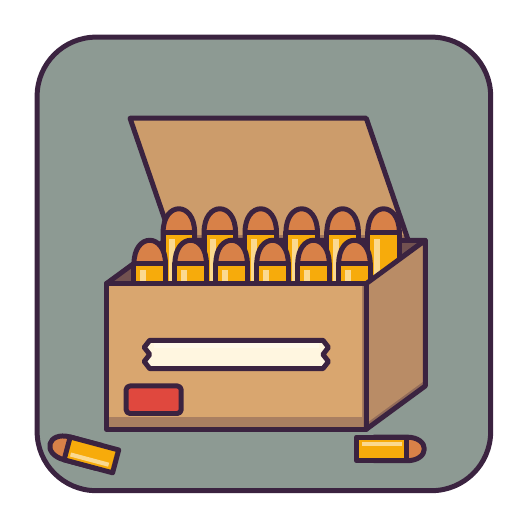
\begin{tikzpicture}
\clip (0,0) rectangle (6,6);
\fill[metal] [rounded corners=0.75cm] (0.12,0.12) rectangle (5.88,5.88);
\begin{scope}\clip [rounded corners=0.75cm] (0.12,0.12) rectangle (5.88,5.88);
\begin{scope}\clip (1.85,3.25) -- (4.85,3.25) -- (4.3,4.85) -- (1.3,4.85) -- cycle;
\fill[woodlight!92!ink!70!ink] (1.85,3.25) -- (4.85,3.25) -- (4.3,4.85) -- (1.3,4.85) -- cycle;
\fill[woodlight!92!ink, shift={(-0.042,0.12)}] (1.85,3.25) -- (4.85,3.25) -- (4.3,4.85) -- (1.3,4.85) -- cycle;
\end{scope}
\draw[inked] (1.85,3.25) -- (4.85,3.25) -- (4.3,4.85) -- (1.3,4.85) -- cycle;
\filldraw[inked, fill=woodlight!35!ink] (1,2.75) -- (4.3,2.75) -- (5.05,3.3) -- (1.75,3.3) -- cycle;
\begin{scope}\clip (1.72,2.85) -- (1.72,3.4) .. controls (1.72,3.8) and (2.12,3.8) .. (2.12,3.4) -- (2.12,2.85) -- cycle;
\fill[orange!55!wood!70!ink] (1.72,2.85) -- (1.72,3.4) .. controls (1.72,3.8) and (2.12,3.8) .. (2.12,3.4) -- (2.12,2.85) -- cycle;
\fill[orange!55!wood, shift={(-0.017,0.05)}] (1.72,2.85) -- (1.72,3.4) .. controls (1.72,3.8) and (2.12,3.8) .. (2.12,3.4) -- (2.12,2.85) -- cycle;
\end{scope}
\draw[inked] (1.72,2.85) -- (1.72,3.4) .. controls (1.72,3.8) and (2.12,3.8) .. (2.12,3.4) -- (2.12,2.85) -- cycle;
\begin{scope}\clip (1.72,2.55) rectangle (2.12,3.4);
\fill[gold!88!wood!70!ink] (1.72,2.55) rectangle (2.12,3.4);
\fill[gold!88!wood, shift={(-0.017,0.05)}] (1.72,2.55) rectangle (2.12,3.4);
\end{scope}
\draw[inked] (1.72,2.55) rectangle (2.12,3.4);
\fill[white, opacity=0.55] (1.8,2.65) rectangle (1.87,3.317);
\begin{scope}\clip (2.24,2.85) -- (2.24,3.4) .. controls (2.24,3.8) and (2.64,3.8) .. (2.64,3.4) -- (2.64,2.85) -- cycle;
\fill[orange!55!wood!70!ink] (2.24,2.85) -- (2.24,3.4) .. controls (2.24,3.8) and (2.64,3.8) .. (2.64,3.4) -- (2.64,2.85) -- cycle;
\fill[orange!55!wood, shift={(-0.017,0.05)}] (2.24,2.85) -- (2.24,3.4) .. controls (2.24,3.8) and (2.64,3.8) .. (2.64,3.4) -- (2.64,2.85) -- cycle;
\end{scope}
\draw[inked] (2.24,2.85) -- (2.24,3.4) .. controls (2.24,3.8) and (2.64,3.8) .. (2.64,3.4) -- (2.64,2.85) -- cycle;
\begin{scope}\clip (2.24,2.55) rectangle (2.64,3.4);
\fill[gold!88!wood!70!ink] (2.24,2.55) rectangle (2.64,3.4);
\fill[gold!88!wood, shift={(-0.017,0.05)}] (2.24,2.55) rectangle (2.64,3.4);
\end{scope}
\draw[inked] (2.24,2.55) rectangle (2.64,3.4);
\fill[white, opacity=0.55] (2.32,2.65) rectangle (2.39,3.317);
\begin{scope}\clip (2.76,2.85) -- (2.76,3.4) .. controls (2.76,3.8) and (3.16,3.8) .. (3.16,3.4) -- (3.16,2.85) -- cycle;
\fill[orange!55!wood!70!ink] (2.76,2.85) -- (2.76,3.4) .. controls (2.76,3.8) and (3.16,3.8) .. (3.16,3.4) -- (3.16,2.85) -- cycle;
\fill[orange!55!wood, shift={(-0.017,0.05)}] (2.76,2.85) -- (2.76,3.4) .. controls (2.76,3.8) and (3.16,3.8) .. (3.16,3.4) -- (3.16,2.85) -- cycle;
\end{scope}
\draw[inked] (2.76,2.85) -- (2.76,3.4) .. controls (2.76,3.8) and (3.16,3.8) .. (3.16,3.4) -- (3.16,2.85) -- cycle;
\begin{scope}\clip (2.76,2.55) rectangle (3.16,3.4);
\fill[gold!88!wood!70!ink] (2.76,2.55) rectangle (3.16,3.4);
\fill[gold!88!wood, shift={(-0.017,0.05)}] (2.76,2.55) rectangle (3.16,3.4);
\end{scope}
\draw[inked] (2.76,2.55) rectangle (3.16,3.4);
\fill[white, opacity=0.55] (2.84,2.65) rectangle (2.91,3.317);
\begin{scope}\clip (3.28,2.85) -- (3.28,3.4) .. controls (3.28,3.8) and (3.68,3.8) .. (3.68,3.4) -- (3.68,2.85) -- cycle;
\fill[orange!55!wood!70!ink] (3.28,2.85) -- (3.28,3.4) .. controls (3.28,3.8) and (3.68,3.8) .. (3.68,3.4) -- (3.68,2.85) -- cycle;
\fill[orange!55!wood, shift={(-0.017,0.05)}] (3.28,2.85) -- (3.28,3.4) .. controls (3.28,3.8) and (3.68,3.8) .. (3.68,3.4) -- (3.68,2.85) -- cycle;
\end{scope}
\draw[inked] (3.28,2.85) -- (3.28,3.4) .. controls (3.28,3.8) and (3.68,3.8) .. (3.68,3.4) -- (3.68,2.85) -- cycle;
\begin{scope}\clip (3.28,2.55) rectangle (3.68,3.4);
\fill[gold!88!wood!70!ink] (3.28,2.55) rectangle (3.68,3.4);
\fill[gold!88!wood, shift={(-0.017,0.05)}] (3.28,2.55) rectangle (3.68,3.4);
\end{scope}
\draw[inked] (3.28,2.55) rectangle (3.68,3.4);
\fill[white, opacity=0.55] (3.36,2.65) rectangle (3.43,3.317);
\begin{scope}\clip (3.8,2.85) -- (3.8,3.4) .. controls (3.8,3.8) and (4.2,3.8) .. (4.2,3.4) -- (4.2,2.85) -- cycle;
\fill[orange!55!wood!70!ink] (3.8,2.85) -- (3.8,3.4) .. controls (3.8,3.8) and (4.2,3.8) .. (4.2,3.4) -- (4.2,2.85) -- cycle;
\fill[orange!55!wood, shift={(-0.017,0.05)}] (3.8,2.85) -- (3.8,3.4) .. controls (3.8,3.8) and (4.2,3.8) .. (4.2,3.4) -- (4.2,2.85) -- cycle;
\end{scope}
\draw[inked] (3.8,2.85) -- (3.8,3.4) .. controls (3.8,3.8) and (4.2,3.8) .. (4.2,3.4) -- (4.2,2.85) -- cycle;
\begin{scope}\clip (3.8,2.55) rectangle (4.2,3.4);
\fill[gold!88!wood!70!ink] (3.8,2.55) rectangle (4.2,3.4);
\fill[gold!88!wood, shift={(-0.017,0.05)}] (3.8,2.55) rectangle (4.2,3.4);
\end{scope}
\draw[inked] (3.8,2.55) rectangle (4.2,3.4);
\fill[white, opacity=0.55] (3.88,2.65) rectangle (3.95,3.317);
\begin{scope}\clip (4.32,2.85) -- (4.32,3.4) .. controls (4.32,3.8) and (4.72,3.8) .. (4.72,3.4) -- (4.72,2.85) -- cycle;
\fill[orange!55!wood!70!ink] (4.32,2.85) -- (4.32,3.4) .. controls (4.32,3.8) and (4.72,3.8) .. (4.72,3.4) -- (4.72,2.85) -- cycle;
\fill[orange!55!wood, shift={(-0.017,0.05)}] (4.32,2.85) -- (4.32,3.4) .. controls (4.32,3.8) and (4.72,3.8) .. (4.72,3.4) -- (4.72,2.85) -- cycle;
\end{scope}
\draw[inked] (4.32,2.85) -- (4.32,3.4) .. controls (4.32,3.8) and (4.72,3.8) .. (4.72,3.4) -- (4.72,2.85) -- cycle;
\begin{scope}\clip (4.32,2.55) rectangle (4.72,3.4);
\fill[gold!88!wood!70!ink] (4.32,2.55) rectangle (4.72,3.4);
\fill[gold!88!wood, shift={(-0.017,0.05)}] (4.32,2.55) rectangle (4.72,3.4);
\end{scope}
\draw[inked] (4.32,2.55) rectangle (4.72,3.4);
\fill[white, opacity=0.55] (4.4,2.65) rectangle (4.47,3.317);
\begin{scope}\clip (1.35,2.45) -- (1.35,3) .. controls (1.35,3.4) and (1.75,3.4) .. (1.75,3) -- (1.75,2.45) -- cycle;
\fill[orange!55!wood!70!ink] (1.35,2.45) -- (1.35,3) .. controls (1.35,3.4) and (1.75,3.4) .. (1.75,3) -- (1.75,2.45) -- cycle;
\fill[orange!55!wood, shift={(-0.017,0.05)}] (1.35,2.45) -- (1.35,3) .. controls (1.35,3.4) and (1.75,3.4) .. (1.75,3) -- (1.75,2.45) -- cycle;
\end{scope}
\draw[inked] (1.35,2.45) -- (1.35,3) .. controls (1.35,3.4) and (1.75,3.4) .. (1.75,3) -- (1.75,2.45) -- cycle;
\begin{scope}\clip (1.35,2.15) rectangle (1.75,3);
\fill[gold!88!wood!70!ink] (1.35,2.15) rectangle (1.75,3);
\fill[gold!88!wood, shift={(-0.017,0.05)}] (1.35,2.15) rectangle (1.75,3);
\end{scope}
\draw[inked] (1.35,2.15) rectangle (1.75,3);
\fill[white, opacity=0.55] (1.43,2.25) rectangle (1.5,2.918);
\begin{scope}\clip (1.87,2.45) -- (1.87,3) .. controls (1.87,3.4) and (2.27,3.4) .. (2.27,3) -- (2.27,2.45) -- cycle;
\fill[orange!55!wood!70!ink] (1.87,2.45) -- (1.87,3) .. controls (1.87,3.4) and (2.27,3.4) .. (2.27,3) -- (2.27,2.45) -- cycle;
\fill[orange!55!wood, shift={(-0.017,0.05)}] (1.87,2.45) -- (1.87,3) .. controls (1.87,3.4) and (2.27,3.4) .. (2.27,3) -- (2.27,2.45) -- cycle;
\end{scope}
\draw[inked] (1.87,2.45) -- (1.87,3) .. controls (1.87,3.4) and (2.27,3.4) .. (2.27,3) -- (2.27,2.45) -- cycle;
\begin{scope}\clip (1.87,2.15) rectangle (2.27,3);
\fill[gold!88!wood!70!ink] (1.87,2.15) rectangle (2.27,3);
\fill[gold!88!wood, shift={(-0.017,0.05)}] (1.87,2.15) rectangle (2.27,3);
\end{scope}
\draw[inked] (1.87,2.15) rectangle (2.27,3);
\fill[white, opacity=0.55] (1.95,2.25) rectangle (2.02,2.918);
\begin{scope}\clip (2.39,2.45) -- (2.39,3) .. controls (2.39,3.4) and (2.79,3.4) .. (2.79,3) -- (2.79,2.45) -- cycle;
\fill[orange!55!wood!70!ink] (2.39,2.45) -- (2.39,3) .. controls (2.39,3.4) and (2.79,3.4) .. (2.79,3) -- (2.79,2.45) -- cycle;
\fill[orange!55!wood, shift={(-0.017,0.05)}] (2.39,2.45) -- (2.39,3) .. controls (2.39,3.4) and (2.79,3.4) .. (2.79,3) -- (2.79,2.45) -- cycle;
\end{scope}
\draw[inked] (2.39,2.45) -- (2.39,3) .. controls (2.39,3.4) and (2.79,3.4) .. (2.79,3) -- (2.79,2.45) -- cycle;
\begin{scope}\clip (2.39,2.15) rectangle (2.79,3);
\fill[gold!88!wood!70!ink] (2.39,2.15) rectangle (2.79,3);
\fill[gold!88!wood, shift={(-0.017,0.05)}] (2.39,2.15) rectangle (2.79,3);
\end{scope}
\draw[inked] (2.39,2.15) rectangle (2.79,3);
\fill[white, opacity=0.55] (2.47,2.25) rectangle (2.54,2.918);
\begin{scope}\clip (2.91,2.45) -- (2.91,3) .. controls (2.91,3.4) and (3.31,3.4) .. (3.31,3) -- (3.31,2.45) -- cycle;
\fill[orange!55!wood!70!ink] (2.91,2.45) -- (2.91,3) .. controls (2.91,3.4) and (3.31,3.4) .. (3.31,3) -- (3.31,2.45) -- cycle;
\fill[orange!55!wood, shift={(-0.017,0.05)}] (2.91,2.45) -- (2.91,3) .. controls (2.91,3.4) and (3.31,3.4) .. (3.31,3) -- (3.31,2.45) -- cycle;
\end{scope}
\draw[inked] (2.91,2.45) -- (2.91,3) .. controls (2.91,3.4) and (3.31,3.4) .. (3.31,3) -- (3.31,2.45) -- cycle;
\begin{scope}\clip (2.91,2.15) rectangle (3.31,3);
\fill[gold!88!wood!70!ink] (2.91,2.15) rectangle (3.31,3);
\fill[gold!88!wood, shift={(-0.017,0.05)}] (2.91,2.15) rectangle (3.31,3);
\end{scope}
\draw[inked] (2.91,2.15) rectangle (3.31,3);
\fill[white, opacity=0.55] (2.99,2.25) rectangle (3.06,2.918);
\begin{scope}\clip (3.43,2.45) -- (3.43,3) .. controls (3.43,3.4) and (3.83,3.4) .. (3.83,3) -- (3.83,2.45) -- cycle;
\fill[orange!55!wood!70!ink] (3.43,2.45) -- (3.43,3) .. controls (3.43,3.4) and (3.83,3.4) .. (3.83,3) -- (3.83,2.45) -- cycle;
\fill[orange!55!wood, shift={(-0.017,0.05)}] (3.43,2.45) -- (3.43,3) .. controls (3.43,3.4) and (3.83,3.4) .. (3.83,3) -- (3.83,2.45) -- cycle;
\end{scope}
\draw[inked] (3.43,2.45) -- (3.43,3) .. controls (3.43,3.4) and (3.83,3.4) .. (3.83,3) -- (3.83,2.45) -- cycle;
\begin{scope}\clip (3.43,2.15) rectangle (3.83,3);
\fill[gold!88!wood!70!ink] (3.43,2.15) rectangle (3.83,3);
\fill[gold!88!wood, shift={(-0.017,0.05)}] (3.43,2.15) rectangle (3.83,3);
\end{scope}
\draw[inked] (3.43,2.15) rectangle (3.83,3);
\fill[white, opacity=0.55] (3.51,2.25) rectangle (3.58,2.918);
\begin{scope}\clip (3.95,2.45) -- (3.95,3) .. controls (3.95,3.4) and (4.35,3.4) .. (4.35,3) -- (4.35,2.45) -- cycle;
\fill[orange!55!wood!70!ink] (3.95,2.45) -- (3.95,3) .. controls (3.95,3.4) and (4.35,3.4) .. (4.35,3) -- (4.35,2.45) -- cycle;
\fill[orange!55!wood, shift={(-0.017,0.05)}] (3.95,2.45) -- (3.95,3) .. controls (3.95,3.4) and (4.35,3.4) .. (4.35,3) -- (4.35,2.45) -- cycle;
\end{scope}
\draw[inked] (3.95,2.45) -- (3.95,3) .. controls (3.95,3.4) and (4.35,3.4) .. (4.35,3) -- (4.35,2.45) -- cycle;
\begin{scope}\clip (3.95,2.15) rectangle (4.35,3);
\fill[gold!88!wood!70!ink] (3.95,2.15) rectangle (4.35,3);
\fill[gold!88!wood, shift={(-0.017,0.05)}] (3.95,2.15) rectangle (4.35,3);
\end{scope}
\draw[inked] (3.95,2.15) rectangle (4.35,3);
\fill[white, opacity=0.55] (4.03,2.25) rectangle (4.1,2.918);
\begin{scope}\clip (1,0.9) -- (4.3,0.9) -- (4.3,2.75) -- (1,2.75) -- cycle;
\fill[woodlight!70!ink] (1,0.9) -- (4.3,0.9) -- (4.3,2.75) -- (1,2.75) -- cycle;
\fill[woodlight, shift={(-0.056,0.16)}] (1,0.9) -- (4.3,0.9) -- (4.3,2.75) -- (1,2.75) -- cycle;
\end{scope}
\draw[inked] (1,0.9) -- (4.3,0.9) -- (4.3,2.75) -- (1,2.75) -- cycle;
\begin{scope}\clip (4.3,0.9) -- (5.05,1.45) -- (5.05,3.3) -- (4.3,2.75) -- cycle;
\fill[woodlight!80!ink!70!ink] (4.3,0.9) -- (5.05,1.45) -- (5.05,3.3) -- (4.3,2.75) -- cycle;
\fill[woodlight!80!ink, shift={(-0.021,0.06)}] (4.3,0.9) -- (5.05,1.45) -- (5.05,3.3) -- (4.3,2.75) -- cycle;
\end{scope}
\draw[inked] (4.3,0.9) -- (5.05,1.45) -- (5.05,3.3) -- (4.3,2.75) -- cycle;
\filldraw[inked,fill=cream] (1.55,1.67) -- (3.75,1.67) -- (3.82,1.76) -- (3.75,1.85) -- (3.82,1.94) -- (3.75,2.03) -- (1.55,2.03) -- (1.48,1.94) -- (1.55,1.85) -- (1.48,1.76) -- cycle;
\fill[white, opacity=0.35] (1.6,1.93) -- (3.7,1.93) -- (3.7,1.99) -- (1.6,1.99) -- cycle;
\begin{scope}\clip[rounded corners=0.05cm] (1.25,1.1) rectangle (1.95,1.45);
\fill[red!70!ink,rounded corners=0.05cm] (1.25,1.1) rectangle (1.95,1.45);
\fill[red,rounded corners=0.05cm, shift={(-0.01,0.03)}] (1.25,1.1) rectangle (1.95,1.45);
\end{scope}
\draw[inked,rounded corners=0.05cm] (1.25,1.1) rectangle (1.95,1.45);
\draw[ink, line width=1.6pt, line cap=round] (1,2.75) -- (4.3,2.75);
\begin{scope}[shift={(4.4,0.65)}, rotate=0, xscale=0.75, yscale=0.75]
\begin{scope}[rotate=-90]
\begin{scope}\clip (-0.2,0) -- (-0.2,0.55) .. controls (-0.2,0.95) and (0.2,0.95) .. (0.2,0.55) -- (0.2,0) -- cycle;
\fill[orange!55!wood!70!ink] (-0.2,0) -- (-0.2,0.55) .. controls (-0.2,0.95) and (0.2,0.95) .. (0.2,0.55) -- (0.2,0) -- cycle;
\fill[orange!55!wood, shift={(-0.017,0.05)}] (-0.2,0) -- (-0.2,0.55) .. controls (-0.2,0.95) and (0.2,0.95) .. (0.2,0.55) -- (0.2,0) -- cycle;
\end{scope}
\draw[inked] (-0.2,0) -- (-0.2,0.55) .. controls (-0.2,0.95) and (0.2,0.95) .. (0.2,0.55) -- (0.2,0) -- cycle;
\begin{scope}\clip (-0.2,-0.3) rectangle (0.2,0.55);
\fill[gold!88!wood!70!ink] (-0.2,-0.3) rectangle (0.2,0.55);
\fill[gold!88!wood, shift={(-0.017,0.05)}] (-0.2,-0.3) rectangle (0.2,0.55);
\end{scope}
\draw[inked] (-0.2,-0.3) rectangle (0.2,0.55);
\fill[white, opacity=0.55] (-0.12,-0.2) rectangle (-0.05,0.468);
\end{scope}
\end{scope}
\begin{scope}[shift={(0.9,0.55)}, rotate=0, xscale=0.75, yscale=0.75]
\begin{scope}[rotate=75]
\begin{scope}\clip (-0.2,0) -- (-0.2,0.55) .. controls (-0.2,0.95) and (0.2,0.95) .. (0.2,0.55) -- (0.2,0) -- cycle;
\fill[orange!55!wood!70!ink] (-0.2,0) -- (-0.2,0.55) .. controls (-0.2,0.95) and (0.2,0.95) .. (0.2,0.55) -- (0.2,0) -- cycle;
\fill[orange!55!wood, shift={(-0.017,0.05)}] (-0.2,0) -- (-0.2,0.55) .. controls (-0.2,0.95) and (0.2,0.95) .. (0.2,0.55) -- (0.2,0) -- cycle;
\end{scope}
\draw[inked] (-0.2,0) -- (-0.2,0.55) .. controls (-0.2,0.95) and (0.2,0.95) .. (0.2,0.55) -- (0.2,0) -- cycle;
\begin{scope}\clip (-0.2,-0.3) rectangle (0.2,0.55);
\fill[gold!88!wood!70!ink] (-0.2,-0.3) rectangle (0.2,0.55);
\fill[gold!88!wood, shift={(-0.017,0.05)}] (-0.2,-0.3) rectangle (0.2,0.55);
\end{scope}
\draw[inked] (-0.2,-0.3) rectangle (0.2,0.55);
\fill[white, opacity=0.55] (-0.12,-0.2) rectangle (-0.05,0.468);
\end{scope}
\end{scope}
\end{scope}
\draw[inked] [rounded corners=0.75cm] (0.12,0.12) rectangle (5.88,5.88);
\end{tikzpicture}
\end{document}
